
Therefore, this work explores some of the challenges of applying neural networks in file fragment classification, attempting to answer the following research questions:

%from pep 4.1
\begin{enumerate}[itemindent=\parindent,label=\textbf{Q\arabic*.}]

    \item How do different neural network models compare to each other in terms of training performance and quality of results for file fragment classification?
    
    \item How does the accuracy of neural network models changes relative to the number of classes in file fragment classification?

    \item Can the inability of the models to distinguish high entropy data from random data explain part of the file fragment classification errors? If so, to what extent?
\end{enumerate}

The initial goal of the first research question was to identify the most promising models on file fragment classification, but an apparent limit was found on how far these models could be improved. This led to the second research question, that explores the influence of the number of classes on the accuracy of the models. While the number of classes seems to influence the accuracy of the trained models, the choice of which file types are included in the dataset has a bigger impact because file types that contain images or use compression were found to have an expressive negative effect on accuracy.
Motivated by these results, the third research question was formulated to test the hypothesis that part of the observed errors is caused by the inability of the models to distinguish high entropy data from random data. These steps are depicted in Figure \ref{fig:steps}.

\todo[inline]{expandir este paragrafo. explicar a Figura 1.1}

\noindent
\begin{figure*}[htb!]
\centering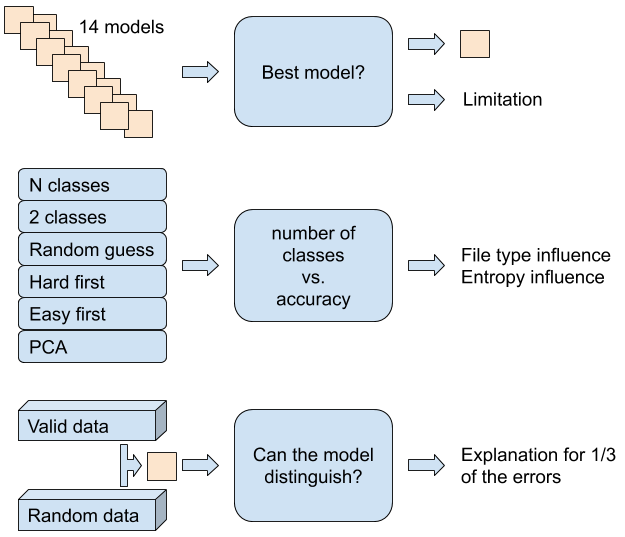
\includegraphics[width=0.8\textwidth]{content/3phases.png}
\caption[Research parts]{\label{fig:steps}Overview of the three parts of the research.}%
\end{figure*}

In this work, only neural networks are taken into account, but other machine learning approaches could also be applied, like Support Vector Machines (SVM) \cite{fitzgerald_using_2012} and k-Nearest Neighbors (kNN) \cite{axelsson_normalised_2010}. This restriction was motivated by the success that neural networks have shown in other fields, like image classification \cite{matan_reading_1992} and speech recognition \cite{graves_speech_2013}.
